%%%%%%%%%%%%%%%%%%%%%%%%%%%%%%%%%%%%%%%%%%%%%%%%%%%%%%%%%%%%%%%%%%%%%%%%%%%%%%%%
%%%%%%%%%%%%%%%%%%%%%%%%%%%%%%%%%%%%%%%%%%%%%%%%%%%%%%%%%%%%%%%%%%%%%%%%%%%%%%%%
\section{Memória}
\index{Aprendizagem!Memória}
\label{sec:memoria}

Memoria se refere ao processo pelo qual um individuo codifica (escreve), 
armazena (retem) e acede (lê) à informação
\cite[pp. 678]{spreen2006compendium} \cite[pp. 31]{de2000comprension}.

Muitos modelos tem sido propostos para explicar a variedade de formas, 
que pode adotar a memória, a Figura \ref{fig:memory-clasification}  mostra um destes modelos
que separa jerarquicamente os diferentes tipos de memória
\cite[pp. 678]{spreen2006compendium}.
Inicialmente a memória é classificada em dois grandes grupos,
a memória de curto prazo e a memória de longo prazo.
\begin{figure}[!h]
  \centering
    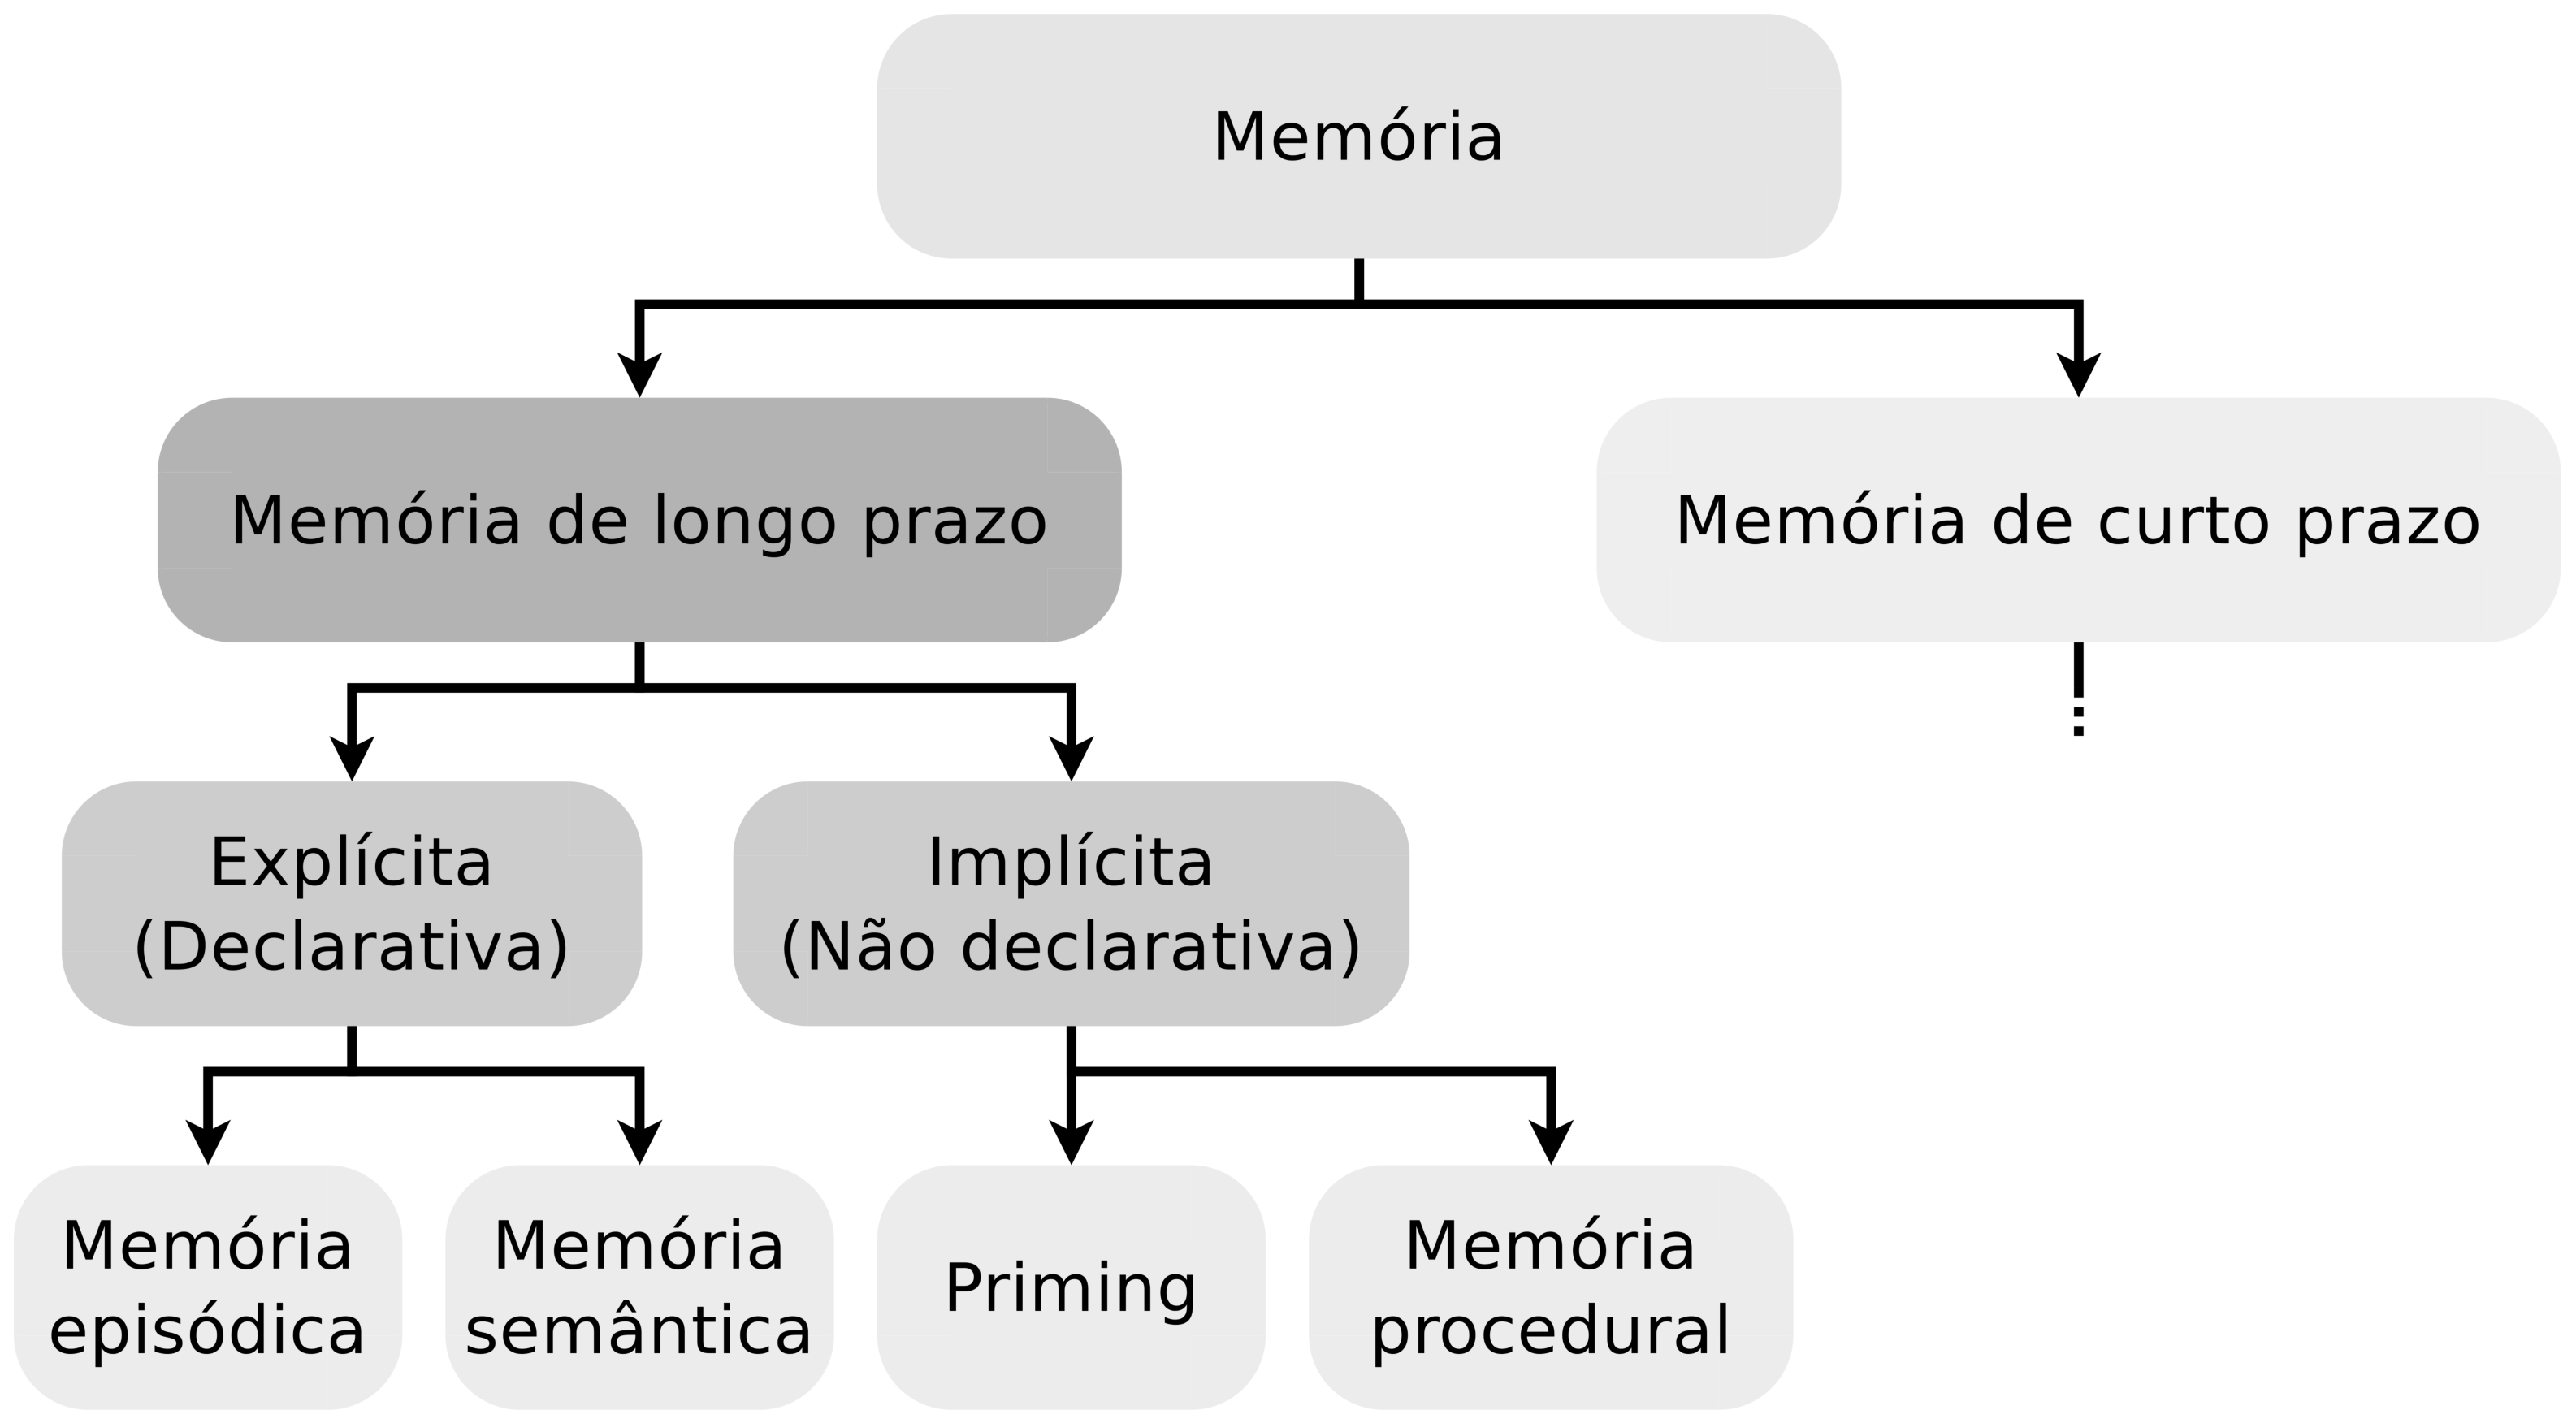
\includegraphics[width=\textwidth]{chapters/cap-learning/memory-clasification.eps} 
  \caption{Hipotética estrutura da memória.}
\label{fig:memory-clasification}
\end{figure}


%%%%%%%%%%%%%%%%%%%%%%%%%%%%%%%%%%%%%%%%%%%%%%%%%%%%%%%%%%%%%%%%%%%%%%%%%%%%%%%%
%%%%%%%%%%%%%%%%%%%%%%%%%%%%%%%%%%%%%%%%%%%%%%%%%%%%%%%%%%%%%%%%%%%%%%%%%%%%%%%%
%%%%%%%%%%%%%%%%%%%%%%%%%%%%%%%%%%%%%%%%%%%%%%%%%%%%%%%%%%%%%%%%%%%%%%%%%%%%%%%%
\subsection{Memória de longo prazo} 
\label{sec:memoria:longo}
Capaz de armazenar uma quantidade grande de informações, 
por períodos de tempos muito longos \cite[pp. 158]{sternbergpsicologia}.
A memória de longo prazo (MLP) contem os saberes, conhecimentos e experiencias obtidas na nossa vida;
esta memória é muito importante para ``compreender'',
pois só compreendemos as coisas que podemos relacionar com coisas conhecidas,
é dizer coisas que já temos na memória de longo prazo \cite[pp. 34]{de2000comprension}.
\begin{example}[Compreendendo objetos:]
Uma ``caneca com doce de pêssego em conserva'', tem sentido pra nos,
porque soubemos que é uma caneca, que é um pêssego e que é um doce em conserva.
\end{example} 

Podemos dividir a memória de longo prazo em dois tipos, 
a memória explícita (declarativa) e 
a memória implícita (não declarativa), ver Figura \ref{fig:implicito-explicito}.
\begin{figure}[!h]
  \centering
    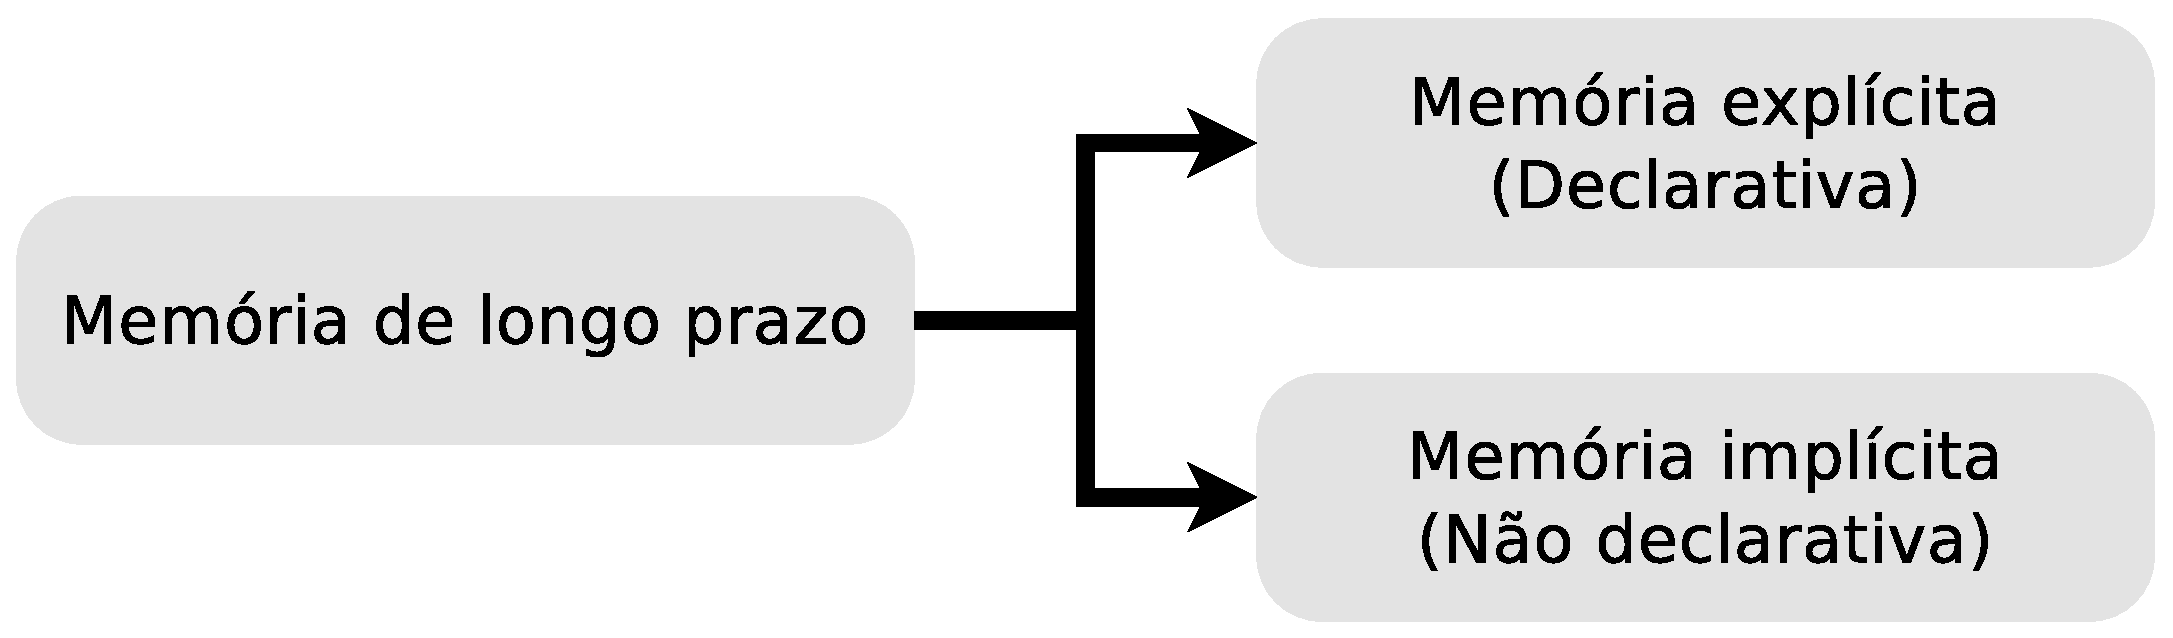
\includegraphics[width=0.8\textwidth]{chapters/cap-learning/memory-mlp.eps} 
  \caption{Tipos de  memória de longo prazo.}
\label{fig:implicito-explicito}
\end{figure}

%%%%%%%%%%%%%%%%%%%%%%%%%%%%%%%%%%%%%%%%%%%%%%%%%%%%%%%%%%%%%%%%%%%%%%%%%%%%%%%%
\subsubsection{Memória explícita (declarativa)} 
\label{subsubsec:explicita}
A memória explicita, também chamada memória declarativa (com informação verbalizável),
é um tipo de memória ``consciente'' que tem informação de todo o relativo a você, 
suas vivencias, e os saberes descontextualizados obtidos ao longo de sua vida
\cite[pp. 138]{pake2019psicologia}.

Podemos dividir a memória explícita em dois tipos, 
a memória episódica e 
a memória semântica, ver Figura \ref{fig:semantica-episodica:explicita}.
\begin{figure}[!h]
  \centering
    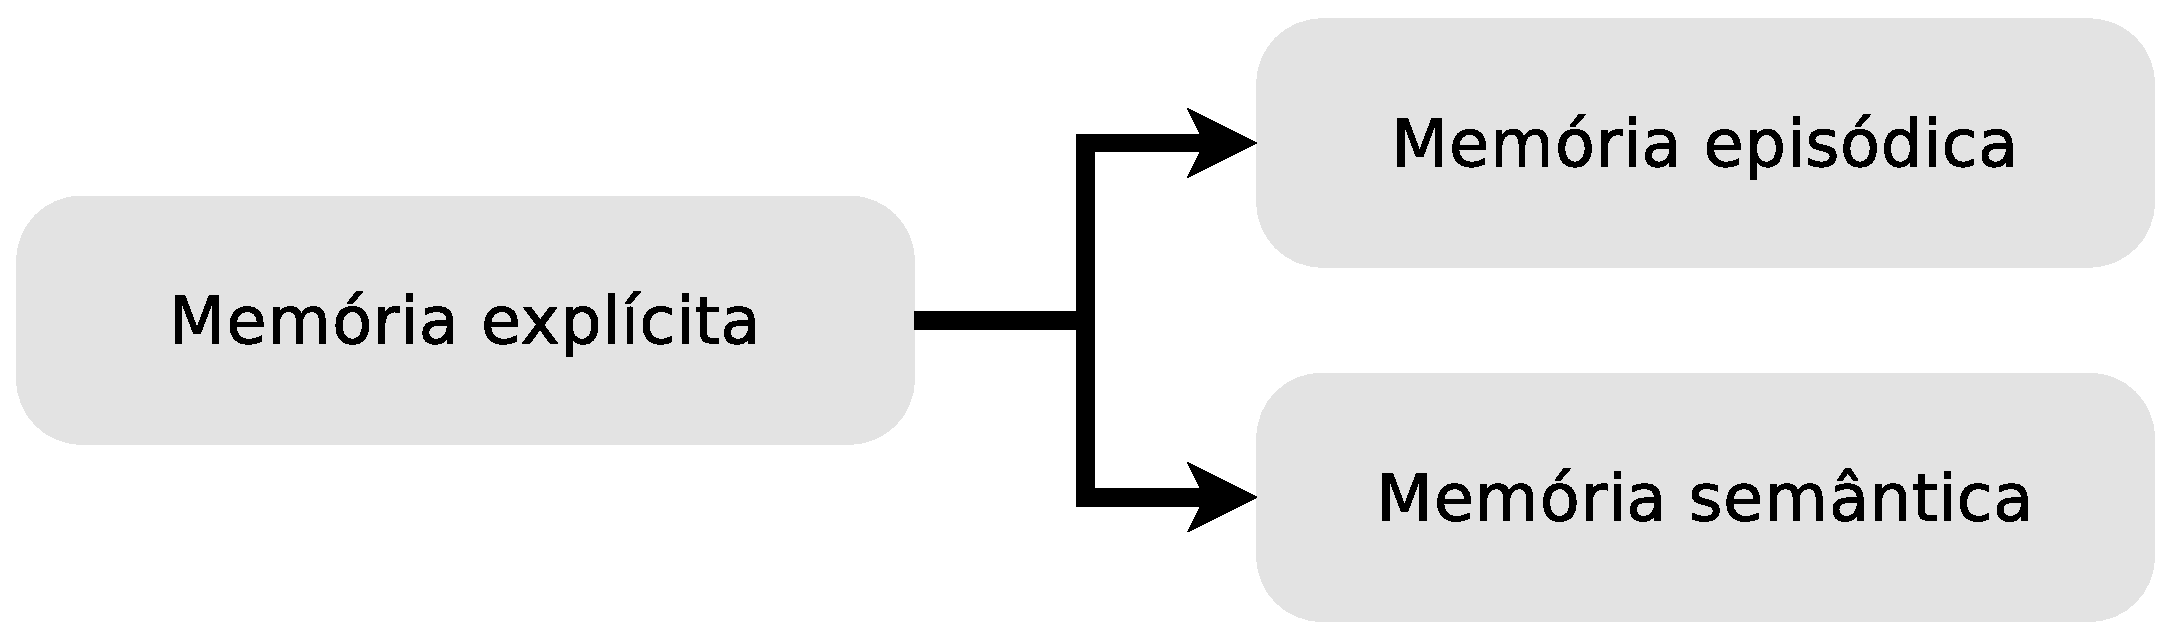
\includegraphics[width=0.7\textwidth]{chapters/cap-learning/memory-explicita.eps} 
  \caption{Tipos de  memória explícita.}
\label{fig:semantica-episodica:explicita}
\end{figure}

\begin{itemize}
%%%%%%%%%%%%%%%%%%%%%%%%%%%%%%%%%%%%%%%%%%%%%%%%%%%%%%%%%%%%%%%%%%%%%%%%%%%%%%%%
\item \textbf{Memória episódica:}  (Episódios, você, donde, quando + emoções)
\label{posref:memoriaepisodica}
Contem lembranças de representações verbais ou sensoriais do experimentado na nossa vida \cite[pp. 138]{pake2019psicologia} \cite[pp. 34-35]{de2000comprension}, 
localizando-os num tempo e espaço específicos;
o conteúdo desta memória é concreto, detalhado, e associado ao contexto que originou a informação,
porém pouco estável e susceptível a modificação; 
pois a memória episódica está tingida de emotividade
\cite[pp. 34-35]{de2000comprension}.
\begin{example}[Contos de marinheiros:]
Quando alguém conta uma aventura marcante na sua vida,
a memória do acontecido e sempre ligeiramente modificada cada vez que esta é contada;
pois é difícil separar o que realmente aconteceu do que nós inconscientemente agregamos quando a evocamos
\cite[pp. 35]{de2000comprension}.
\end{example}
A  evocação na memória episódica é através de representações verbais e imagens visuais
\cite[pp. 35]{de2000comprension}.
A memória episódica não só armazena momentos vividos, 
e sim também historias que tenhamos lido, escutado ou visto
\cite[pp. 35]{de2000comprension}.
\begin{example}[Lembrando palestra:]
Quando participamos e conseguimos lembrar de uma palestra, 
é porque a informação passou a formar parte da memória episódica;
porém sua permanência é precária, 
pois geralmente esta  informação não tem o componente emocional necessário para garantir sua permanência.
Assim, uma forma de fixar permanentemente a informação percebida na memória episódica,
é agregando um componente emocional cada vez que recebemos este tipo de informação.
\end{example}
%%%%%%%%%%%%%%%%%%%%%%%%%%%%%%%%%%%%%%%%%%%%%%%%%%%%%%%%%%%%%%%%%%%%%%%%%%%%%%%%
\item \textbf{Memória semântica:} (Conceitos, significados, mundo, estruturas)
\label{posref:memoriasemantica}
Armazena todos os conceitos e saberes culturais do mundo aprendidos ao longo da vida 
\cite[pp. 139]{pake2019psicologia} \cite[pp. 34]{de2000comprension},
convenientemente descontextualizados em tempo e espaço para seu armazenamento;
toda esta informação (conhecimentos) provem do vocabulário que adquirimos a medida que aprendemos nossa língua e cultura
\cite[pp. 34]{de2000comprension}.
Toda esta informação se encontra armazenada formando estruturas relacionais, 
de ali vem a facilidade com que esta informação é evocada
\cite[pp. 34]{de2000comprension};
a  evocação na memória semântica é através de representações verbais
\cite[pp. 35]{de2000comprension}.
\begin{example}[Reconhecendo uma caneca:]
Provavelmente nós possamos souber que é uma caneca, 
porém é pouco provável que lembremos quando e como aprendemos esta informação.
O que sim temos  certeza é que a caneca está emparentada com os copos, e que existem canecas de diversos tipos.
\end{example}
As memórias semânticas tendem a ser mais estáveis que as memorias episódicas,
pois tem um uso frequente, o que reforça sua estabilidade \cite[pp. 140]{pake2019psicologia}.
\end{itemize}


%%%%%%%%%%%%%%%%%%%%%%%%%%%%%%%%%%%%%%%%%%%%%%%%%%%%%%%%%%%%%%%%%%%%%%%%%%%%%%%%
\subsubsection{Memória implícita (não declarativa)} 
\label{subsubsec:implicita}
A memória implícita, também chamada memória não declarativa (com informação não verbalizável),
é um tipo de memória ``inconsciente''
\cite[pp. 140]{pake2019psicologia}.

Podemos dividir a memória implícita nos seguintes tipos, 
a memória procedural e 
a memória ``priming'', ver Figura \ref{fig:semantica-episodica}.
\begin{figure}[!h]
  \centering
    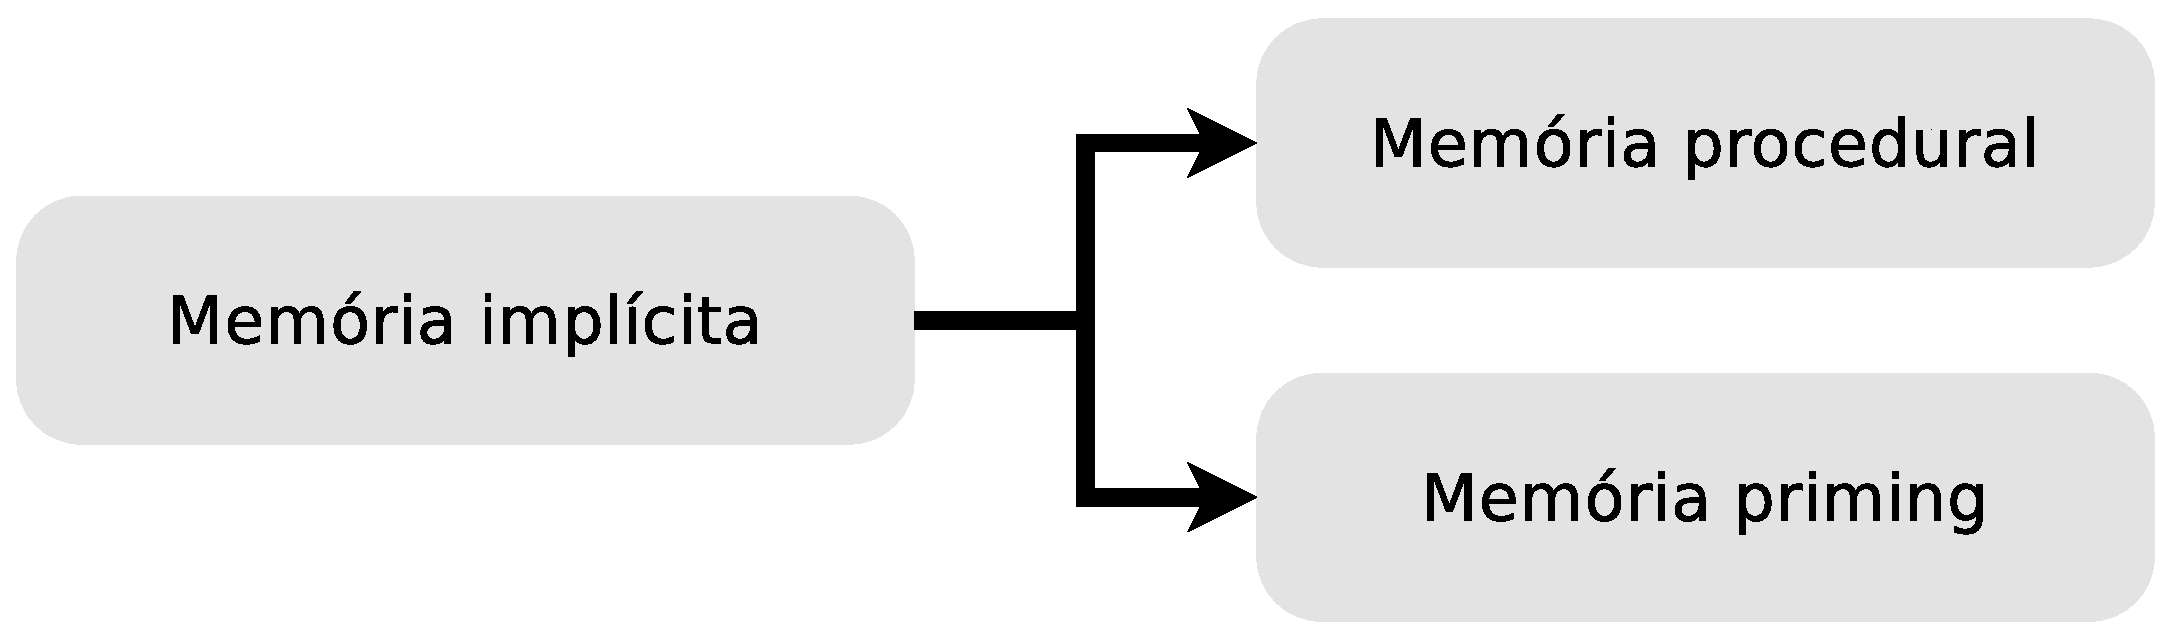
\includegraphics[width=0.7\textwidth]{chapters/cap-learning/memory-implicita.eps} 
  \caption{Tipos de  memória implícita.}
\label{fig:semantica-episodica}
\end{figure}

\begin{itemize}
%%%%%%%%%%%%%%%%%%%%%%%%%%%%%%%%%%%%%%%%%%%%%%%%%%%%%%%%%%%%%%%%%%%%%%%%%%%%%%%%
\item \textbf{Memória procedural:}
\label{reflab:memprocedural}
Os seres humanos desenvolvemos, ao longo do tempo, ``destrezas para executar uma ação ou procedimento'';
é dizer habilidades
\cite[pp. 140]{pake2019psicologia} \cite[pp. 36]{de2000comprension}.
\begin{example}[Ações e procedimentos:]
Usar a bicicleta, dirigir, escrever, desenhar, comer, nadar, fazer a cama \cite[pp. 36]{de2000comprension},
procedimentos matemáticos \cite{evans2016extension} \cite{davis2000memory}.
\end{example}
Mesmo que não tenhamos praticado a atividade por muito tempo, 
basta que iniciemos a ação para que nossa antiga habilidade se reatualize 
\cite[pp. 36]{de2000comprension}.
O conhecimento proveniente da memória procedural é difícil de verbalizar
\cite[pp. 36]{de2000comprension}, pelo que entra na categoria de não declarativa.
\begin{example}[Ensinando geometria:]
Quando estudas geometria, 
muitas vezes a solução a um problema é obtida rapidamente quando realizamos o procedimento de agregar um traço auxiliar;
porém, para algumas pessoas parece natural souber onde realizar esta modificação ao problema,
pois por sua experiencia, para eles é natural souber onde deve ser colocada o traço auxiliar;
pelo que para eles é difícil explicar aos demais quais foram os mecanismos que provocaram essa escolha,
e só podem ensinar a efetividade de realizar essa escolha.

A Figura \ref{fig:geometria:a} representa um exemplo de um problema geométrico, 
onde a pergunta é achar o angulo $\alpha$. 
A Figura \ref{fig:geometria:b} mostra
como o problema pode ser facilmente solucionado agregando um traço auxiliar 
prudente e intuitivamente escolhido.
\end{example}
\begin{figure}[!h]
  \centering
     \begin{subfigure}[b]{0.4\textwidth}
         \centering
         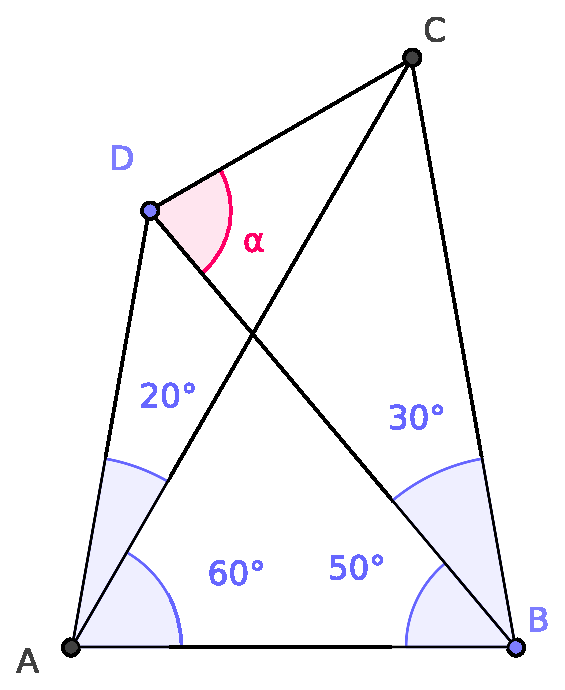
\includegraphics[width=0.95\textwidth]{chapters/cap-learning/prob-geometria1.eps} 
         \caption{Problema geométrico.}
         \label{fig:geometria:a}
     \end{subfigure}
     \hfill
     \begin{subfigure}[b]{0.4\textwidth}
         \centering
         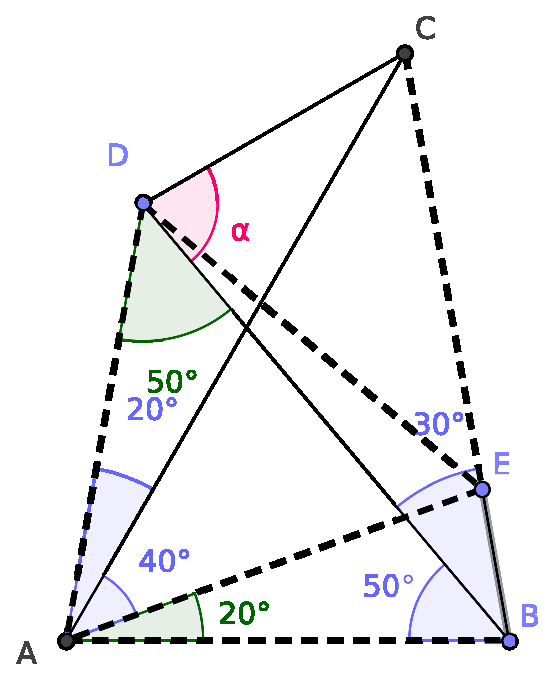
\includegraphics[width=0.95\textwidth]{chapters/cap-learning/prob-geometria2.eps} 
         \caption{Traço auxiliar.}
         \label{fig:geometria:b}
     \end{subfigure}
  \caption{Resolução de um problema geométrico.}
\label{fig:geometria}
\end{figure}

As repetições das ações levam ao fortalecimento da memória procedural
\cite[pp. 36]{de2000comprension};
quando as pessoas iniciam a aprender uma nova tarefa, 
estas dependem geralmente da sua 
\hyperref[posref:memoriaepisodica]{\textbf{memoria episódica}} e 
\hyperref[posref:memoriasemantica]{\textbf{semântica}};
e dizer a memória \hyperref[subsubsec:explicita]{\textbf{declarativa}}; 
porém com o tempo todas essas tarefas são sintetizadas numa única tarefa procedural,
virando natural em nós e provavelmente difícil de verbalizar (não declarativa) e expor como fazemos ela
 \cite[pp. 141]{pake2019psicologia}.
\begin{example}[Aprendendo a trança:]
Quando nos foi ensinado o movimento da trança, 
nós decoramos os movimentos e a ordem deles;
esta informação foi armazenada provavelmente provavelmente em algum lugar da  
\hyperref[subsubsec:explicita]{\textbf{memória declarativa}},
já seja na memória episódica (se o professor criou um ambiente marcante emocionalmente)
ou na memória semântica (se o professor teve a habilidade pedagógica de fixar na memória cada parte do movimento);
porém com muito tempo de treino que envolve varias repetições,
esta informação foi conformando-se numa única tarefa procedural (memoria procedural), a "trança",
 que não precisava de muita de nossa atenção\footnote{Devemos ter cuidado que neste processo,
a informação na memoria declarativa tende a perde-se por falta de uso, 
isto poderia ser pouco importante sim só queremos dançar, 
porém é um problema sim queremos ou devemos ensinar este movimento aos demais.}.
\end{example}

%%%%%%%%%%%%%%%%%%%%%%%%%%%%%%%%%%%%%%%%%%%%%%%%%%%%%%%%%%%%%%%%%%%%%%%%%%%%%%%%
\item \textbf{Memória ``priming'' (representação):}
Também chamada memória de representação, 
este é uma forma rápida para o aprendizado inconsciente;
onde cada acesso a informação influencia o processamento desta informação a seguinte vez que é evocada
\cite[pp. 141]{pake2019psicologia}.
\begin{example}[Pular:]
Se numa aula de dança introduzimos a uma pessoa o conceito de pular num determinado movimento, 
quando nessa aula usemos novamente o conceito de pular em outro movimento, 
para esta pessoa será mais fácil processar e atuar seguindo esta ideia.
\end{example}

O priming também é conhecido por ativar áreas cerebrais afins ao assunto sendo representado
\cite[pp. 142]{pake2019psicologia}
\begin{example}[Gancho redondo:]
Se evocamos um movimento de dança como o gancho redondo;
então são ativadas regiões cerebrais associadas ao gancho redondo, 
gancho (simples) e temas afins como o puladinho.
\end{example}

\end{itemize}

%%%%%%%%%%%%%%%%%%%%%%%%%%%%%%%%%%%%%%%%%%%%%%%%%%%%%%%%%%%%%%%%%%%%%%%%%%%%%%%%
%%%%%%%%%%%%%%%%%%%%%%%%%%%%%%%%%%%%%%%%%%%%%%%%%%%%%%%%%%%%%%%%%%%%%%%%%%%%%%%%
%%%%%%%%%%%%%%%%%%%%%%%%%%%%%%%%%%%%%%%%%%%%%%%%%%%%%%%%%%%%%%%%%%%%%%%%%%%%%%%%
\subsection{Memória de curto prazo } 
\label{sec:memoria:curto}



Esta memória é capaz de armazenar de forma limitada, 
informações por períodos de tempo que vão desde segundos ate 1-2 minutos
\cite[pp. 678]{spreen2006compendium} \cite[pp. 158]{sternbergpsicologia}.
A informação que carregamos na memória de curto prazo (MCP),
seguindo o modelo visto na Figura \ref{fig:sentidos-memoria},  
pode provir de duas fontes de informação, do \hyperref[fig:sentidos-memoria]{\textbf{registro sensorial}} 
ou da \hyperref[sec:memoria:longo]{\textbf{memória de longo prazo}}.


O termo mais usado atualmente para designar a este tipo de memória é 
\hyperref[subsubsec:memoriatrabalho]{\textbf{memória de trabalho}},
substituindo assim aos termos mais antigos como ``memória de curto prazo'' ou ``memória imediata''
\cite[pp. 678]{spreen2006compendium}.
Porém alguns autores indicam  que, mesmo considerando-se próximos, 
existem diferenças entre o modelo proposto pelo termo 
``memória de trabalho'' e o proposto pelo termo ``memória de curto prazo'' 
\cite[pp. 266, 267, 269]{braisby2012cognitive};
pois o termo memória de trabalho indica que além de armazenar informações por um curto período de tempo
esta também realiza operações sobre as informações evocadas; 
por exemplo, realizar mentalmente operações matemáticas com acumulação de resultados 
\cite[pp. 267, 272]{braisby2012cognitive}.


%%%%%%%%%%%%%%%%%%%%%%%%%%%%%%%%%%%%%%%%%%%%%%%%%%%%%%%%%%%%%%%%%%%%%%%%%%%%%%%%
\subsubsection{Memória de trabalho} 
\label{subsubsec:memoriatrabalho}

\begin{wrapfigure}{r}{0.38\textwidth}
  \centering
    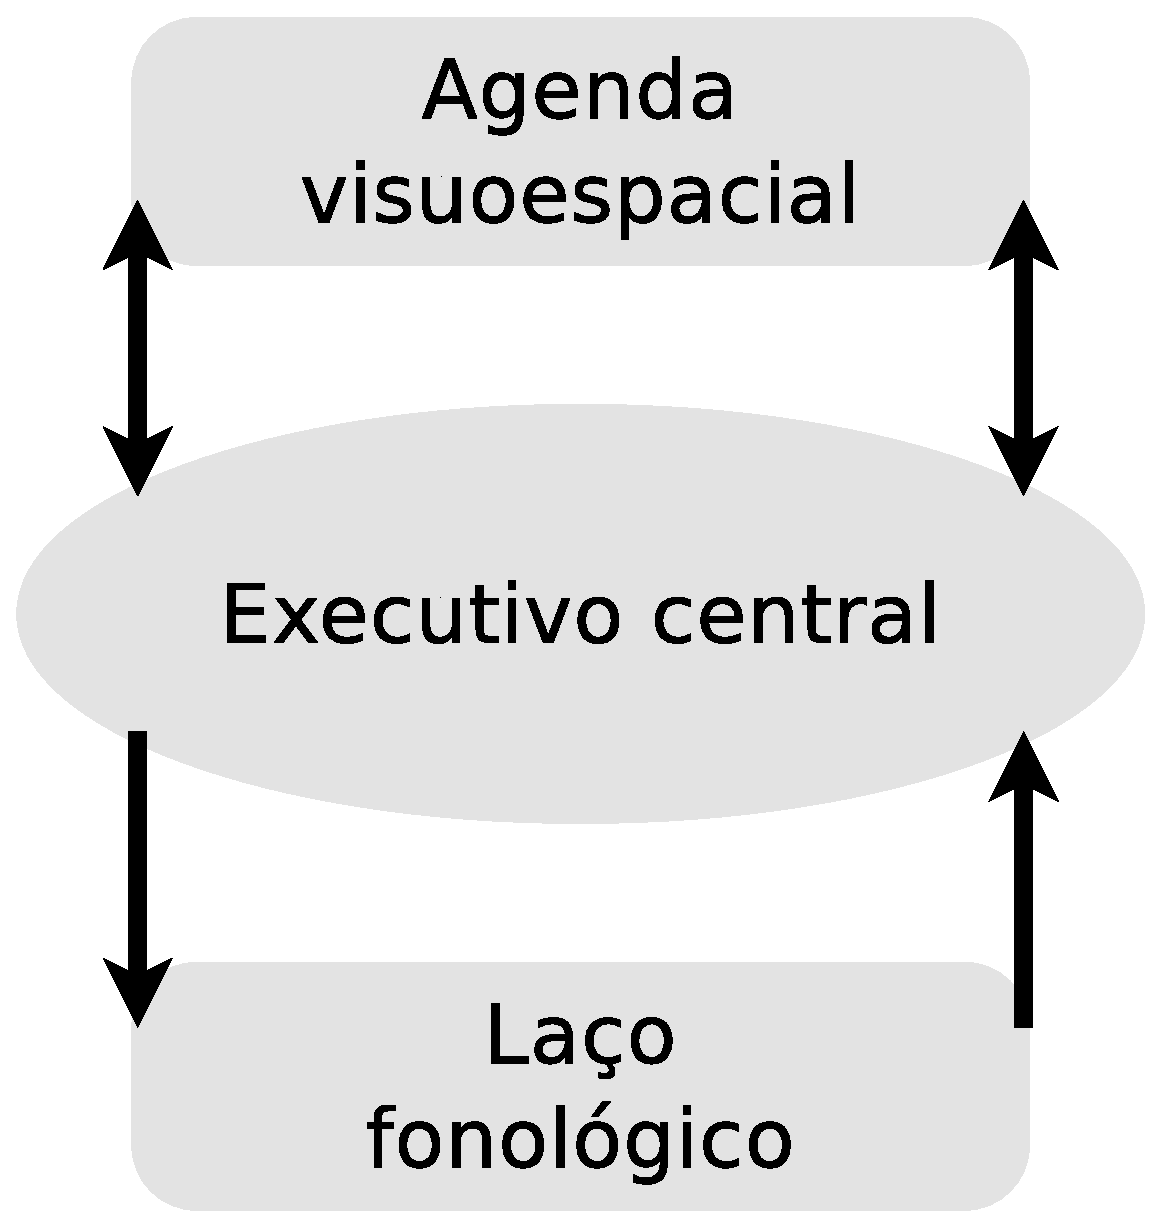
\includegraphics[width=0.33\textwidth]{chapters/cap-learning/memory-mcp.eps}
\caption{Modelo de memória de trabalho.}
\label{fig:memory-mcp}
\end{wrapfigure}
A memória de trabalho nos ajuda a ter temporariamente informações para a toma de decisões nas
nossas atividades (planejar, aprender, raciocinar, resolver problemas e seguir instruções),
ate que novas informações sejam recebidas 
\cite[pp. 678]{spreen2006compendium} \cite[pp. 266]{braisby2012cognitive}.
A memória de trabalho também atua para manter as informações ativas e disponíveis,
 ate que estas possam ser enviadas à memória de longo prazo
\cite[pp. 678]{spreen2006compendium}.

O modelo mais reconhecido da memória de trabalho foi proposto por Baddeley e Hitch  (1974)
e Baddeley (1983; 1986), como mostra a Figura \ref{fig:memory-mcp},
onde podemos apreciar um sistema de  supervisão e controle (executivo central),
e dois sistemas periféricos escravos:
o laço ou ciclo fonológico (ou articulatório) e a agenda visuoespacial
\cite[pp. 678]{spreen2006compendium} \cite[pp. 266, 272, 273]{braisby2012cognitive}.
Baddeley em anos posteriores redefiniu seu modelo agregando um novo componente, 
o buffer episódico \cite[pp. 284]{braisby2012cognitive} \cite[pp. 678]{spreen2006compendium} \cite[pp. 122]{pake2019psicologia},
como pode ser visto na Figura \ref{fig:memory-working}.
\begin{figure}[!h]
  \centering
    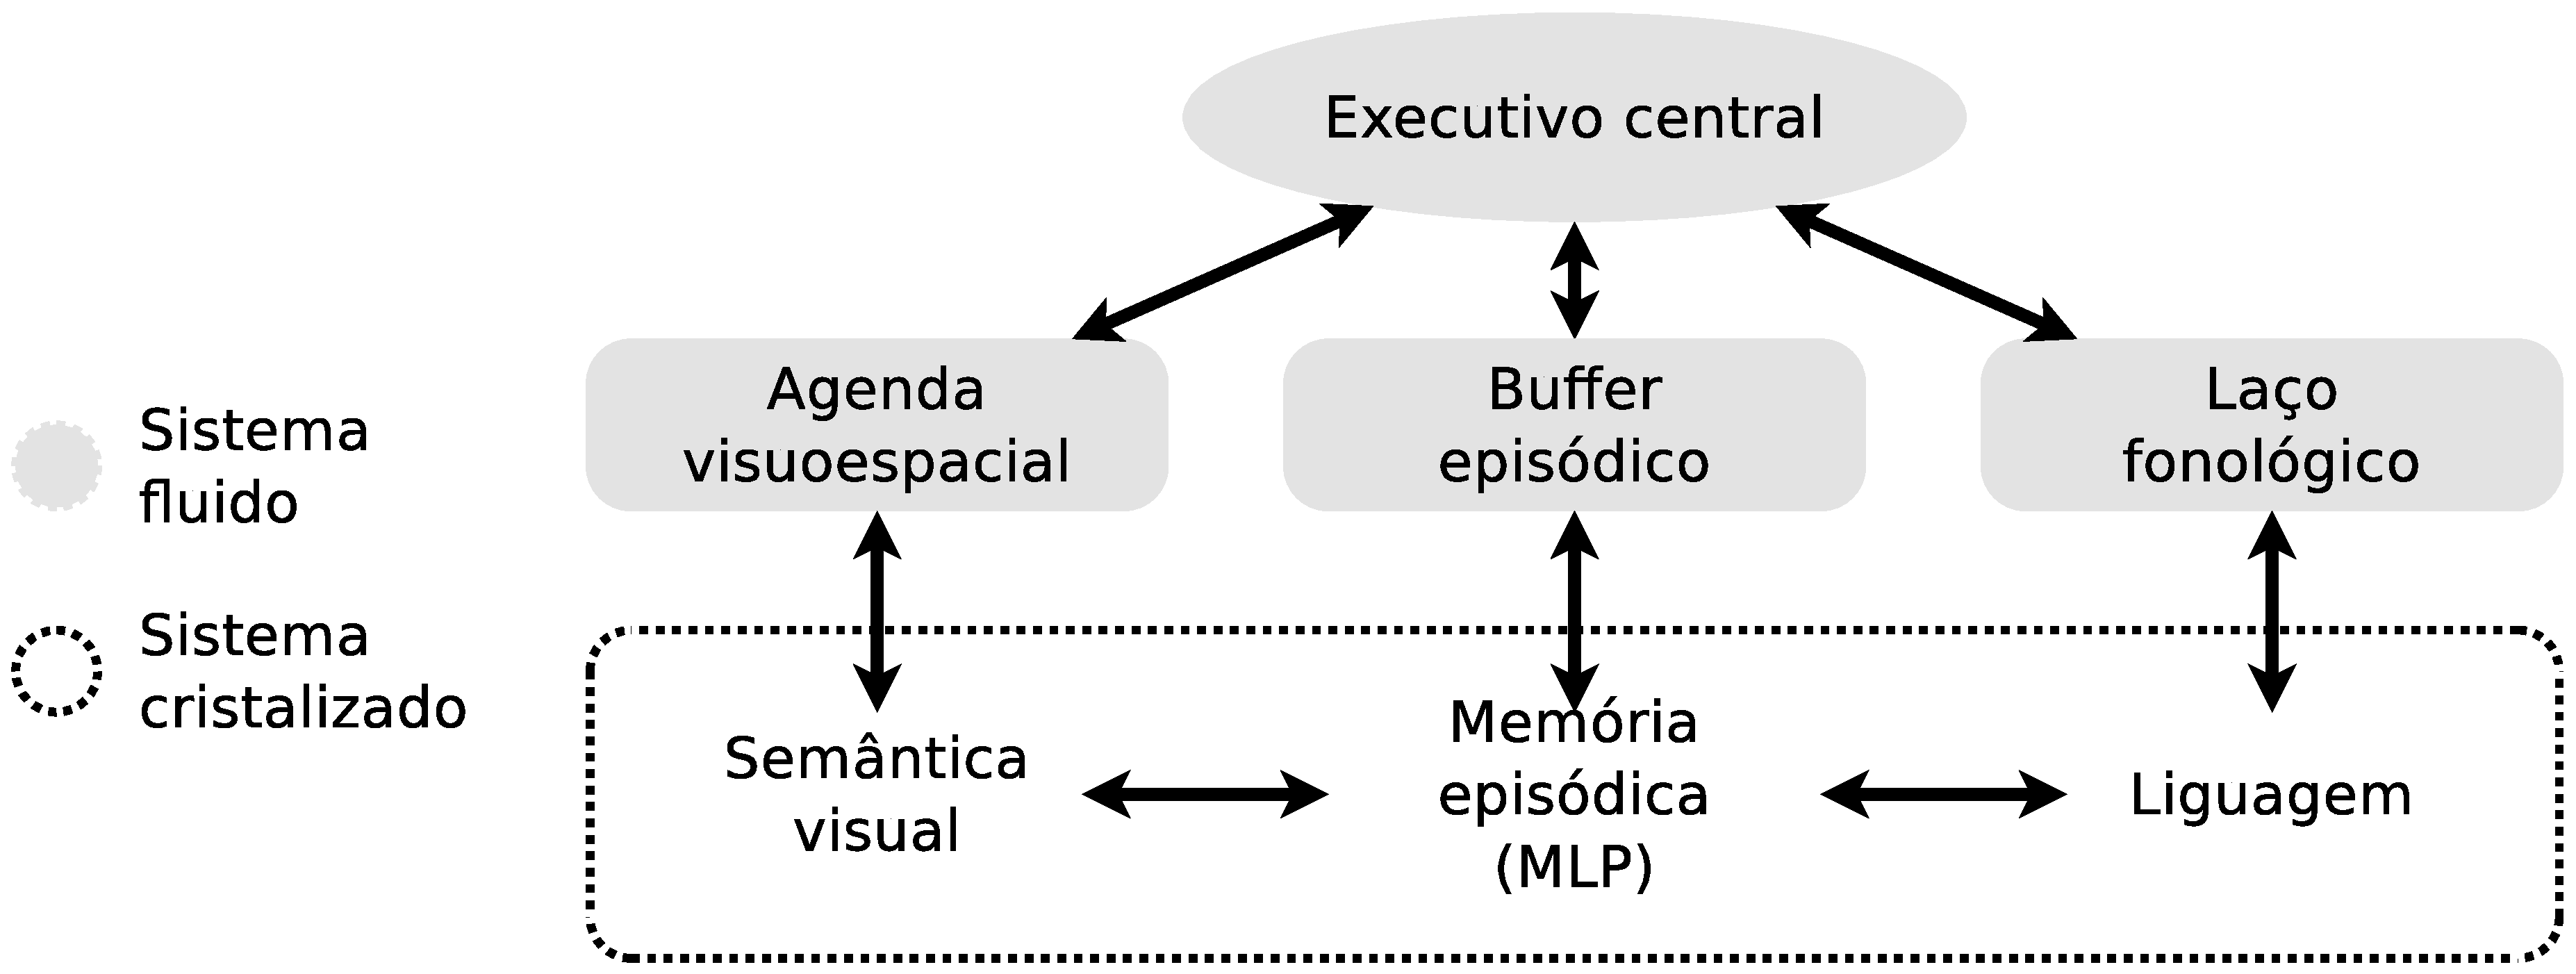
\includegraphics[width=0.99\textwidth]{chapters/cap-learning/memory-working.eps}
\caption{Modelo revisado da memória de trabalho.}
\label{fig:memory-working}
\end{figure}

\begin{description}

\item[Executivo central:]
\label{reflabel:executivocentral}
O executivo central controla tarefas visuais e verbais; 
porém, tem um subsistema separado para armazenar informação visuoespacial 
\cite[pp. 273]{braisby2012cognitive} como mostram as Figura \ref{fig:memory-mcp} e \ref{fig:memory-working}.
O executivo central  é o responsável por supervisionar, 
controlar e coordenar os outros sistemas, 
formando estratégias para usar as informações que eles contêm,
facilitando assim atividades cognitivas complexas como o aprendizado, a compreensão e o raciocínio
\cite[pp. 272]{braisby2012cognitive} \cite[pp. 678]{spreen2006compendium} \cite[pp. 126]{pake2019psicologia}.
Este é conceituado como um sistema de supervisão de atenção com capacidade limitada
\cite[pp. 272, 281]{braisby2012cognitive} \cite[pp. 678]{spreen2006compendium}
com vários subcomponentes que ainda não foram claramente definidos e entendidos
\cite[pp. 285]{braisby2012cognitive}.


\item[Laço fonológico:] (armazena informação vinculando-o a um sonido)
\label{reflabel:fonologico}
O laço fonológico é geralmente descrito como o ouvido da mente ou como a nossa voz interior \cite[pp. 122]{pake2019psicologia}, 
e está encarregado de armazenar temporariamente pequenas quantidades de informação, 
de material baseado em sons (ex:fala), durante processos cognitivos
sem afetar ao ``executivo central'' 
\cite[pp. 678]{spreen2006compendium} \cite[pp. 272]{braisby2012cognitive} \cite[pp. 122]{pake2019psicologia};
porém, carregar grandes quantidades de informação ocuparia sim, recursos extras do ``executivo central''
\cite[pp. 272]{braisby2012cognitive}.
A estrutura do laço fonológico seguindo o modelo proposto por Baddeley (1984) pode ser visto na Figura  \ref{fig:lacofonologico}
\cite[pp. 276]{braisby2012cognitive}.
Tarefas como o ``digit span''\footnote{``digit span'' é a lista mais longa de dígitos que uma 
pessoa pode repetir (evocar) na ordem correta.} são gerenciadas principalmente pelo laço fonológico 
\cite[pp. 678]{spreen2006compendium}.
Assim, o laço fonológico ocupa um lugar essencial no desenvolvimento de nossas habilidades intelectuais. 
\begin{figure}[!h]
  \centering
    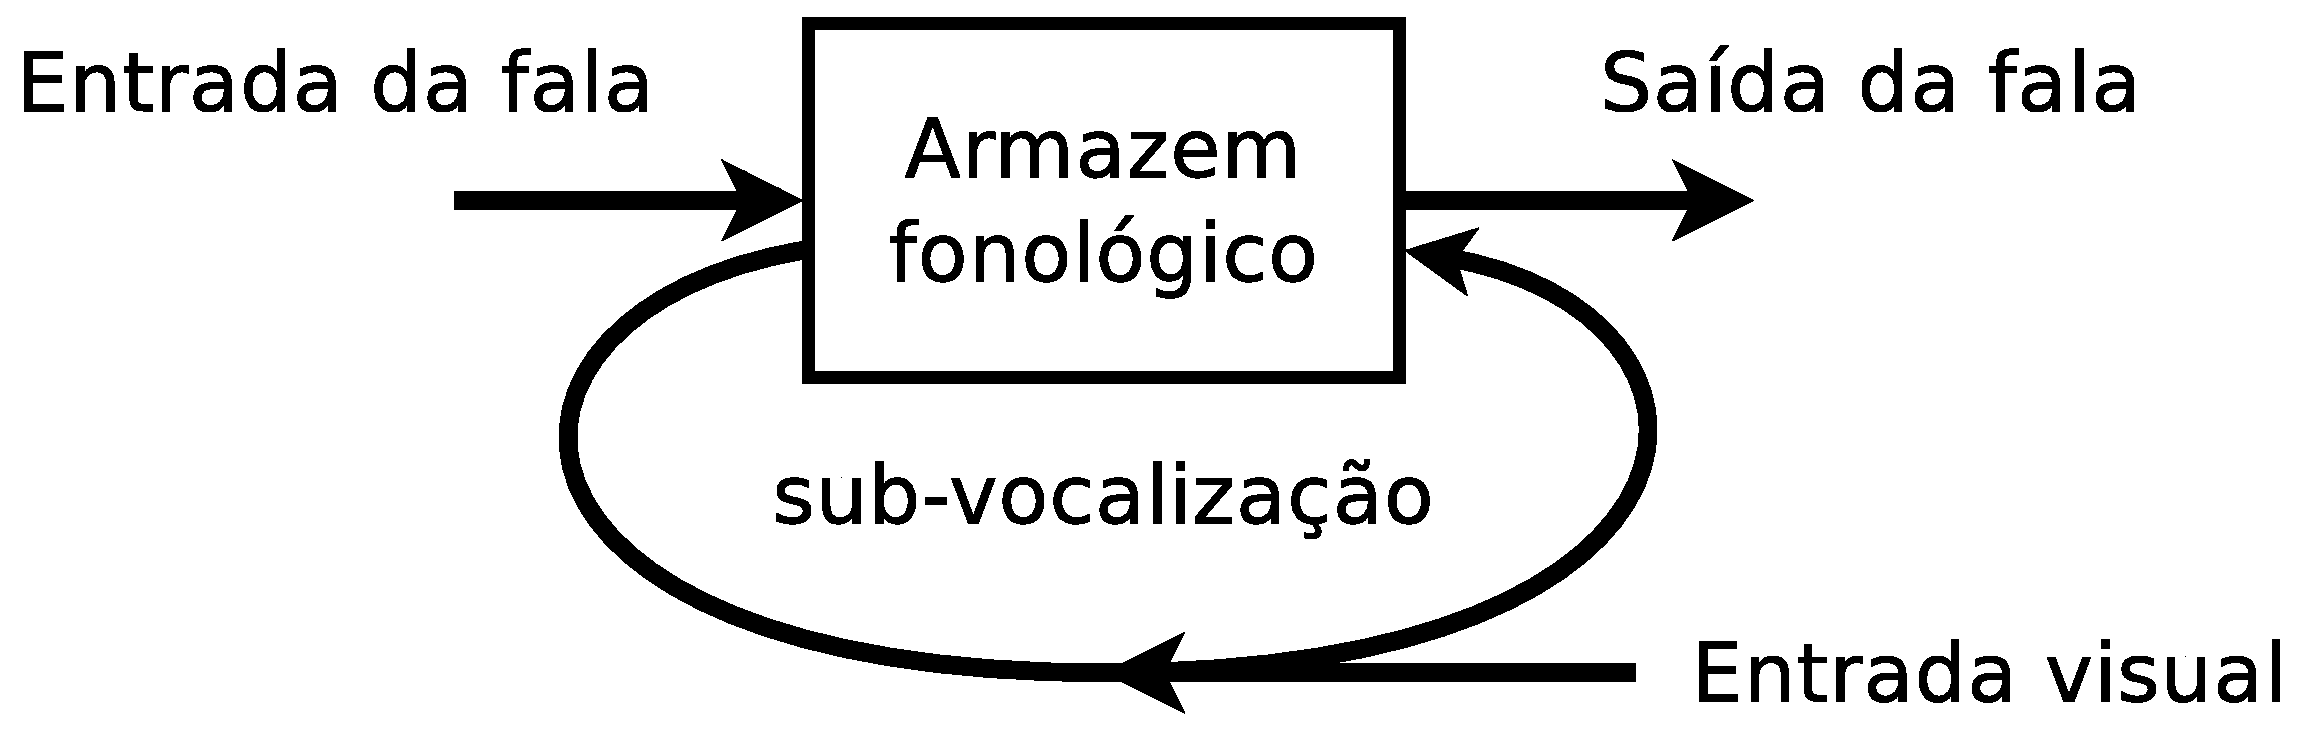
\includegraphics[width=0.7\textwidth]{chapters/cap-learning/fonologico.eps}
\caption{Estrutura do laço fonológico.}
\label{fig:lacofonologico}
\end{figure}

\item[Agenda visuoespacial:] (armazena informação vinculando-o a uma imagem)
\label{reflabel:visuoespacial}
A agenda visuoespacial está encarregado de armazenar temporariamente  e processar pequenas quantidades de informação
de material baseado em visão (ex: Imagens mentais) e informação espacial
\cite[pp. 678]{spreen2006compendium} \cite[pp. 124]{pake2019psicologia};
porém, as informações são separadas numa memória  espacial e uma memória visual \cite[pp. 124]{pake2019psicologia}.
%Este sistema está dividido num componente espacial e outro visual
%um possível componente cinestésico na memória de trabalho não tem sido ainda estabelecido
%\cite[pp. 274, 285]{braisby2012cognitive}.
A combinação de  subsistemas espaciais e visuais conformam um sistema de movimento no espaço, 
que é usado para lembrar sequencia de ações e assim aprender habilidades motoras;
estas informações a sua vez podem ser usadas para atualizar o conteúdo do armazém de informação visual
(onde estou? que me falta? que faço agora?)
\cite[pp. 274]{braisby2012cognitive} \cite[pp. 125]{pake2019psicologia}.
Tarefas como o ``spatial span''\footnote{``spatial span'' é a lista mais longa de posições que uma 
pessoa pode repetir (evocar) na ordem correta.} 
são gerenciadas principalmente pela agenda visuoespacial 
\cite[pp. 678]{spreen2006compendium}.
Assim a agenda visuoespacial nos permite perceber os objetos, 
encontrar endereços ou realizar jogos onde exista movimento realizado por nós ou pelo objeto lúdico. 


\item[Buffer episódico:] 
Este é um lugar de armazenamento com capacidade limitada que une informações em 
pequenos pedaços para formar episódios integrados 
\cite[pp. 678]{spreen2006compendium} \cite[pp. 126]{pake2019psicologia}.
O buffer episódico conecta a MLP com a memória de trabalho, 
fazendo de ponte no fluxo de informação e ambos sentidos;
além de atuar como um deposito temporário das informações da MLP
trazendo esta informação a percepção consciente
\cite[pp. 126]{pake2019psicologia} \cite[pp. 283-284]{braisby2012cognitive}.
Como pode ser visto no diagrama da Figura \ref{fig:lacofonologico}, 
o buffer episódico também permite conectar as informações do laço fonológico e da agenda visuoespacial
\end{description}
